\documentclass[9pt]{beamer}

% Beamer style
%\usetheme[secheader]{Madrid}
% \usetheme{CambridgeUS}
\useoutertheme{infolines}
\usecolortheme[rgb={0.65,0.15,0.25}]{structure}
% \usefonttheme[onlymath]{serif}
\beamertemplatenavigationsymbolsempty
%\AtBeginSubsection

% Packages
%\usepackage[french]{babel}
\usepackage[latin1]{inputenc}
\usepackage{color}
% \usepackage[dvipsnames]{xcolor}
\usepackage{xspace}
\usepackage{dsfont, stmaryrd}
\usepackage{amsmath, amsfonts, amssymb, stmaryrd, mathabx}
\usepackage{epsfig}
\usepackage{tikz}
\usepackage{url}
% \usepackage{ulem}
\usepackage{/home/robin/LATEX/Biblio/astats}
%\usepackage[all]{xy}
\usepackage{graphicx}

% Maths
% \newtheorem{theorem}{Theorem}
% \newtheorem{definition}{Definition}
\newtheorem{proposition}{Proposition}
% \newtheorem{assumption}{Assumption}
% \newtheorem{algorithm}{Algorithm}
% \newtheorem{lemma}{Lemma}
% \newtheorem{remark}{Remark}
% \newtheorem{exercise}{Exercise}
% \newcommand{\propname}{Prop.}
% \newcommand{\proof}{\noindent{\sl Proof:}\quad}
% \newcommand{\eproof}{$\blacksquare$}

% \setcounter{secnumdepth}{3}
% \setcounter{tocdepth}{3}
\newcommand{\pref}[1]{\ref{#1} p.\pageref{#1}}
\newcommand{\qref}[1]{\eqref{#1} p.\pageref{#1}}

% Colors : http://latexcolor.com/
\definecolor{darkred}{rgb}{0.65,0.15,0.25}
\definecolor{darkgreen}{rgb}{0,0.4,0}
\definecolor{darkred}{rgb}{0.65,0.15,0.25}
\definecolor{amethyst}{rgb}{0.6, 0.4, 0.8}
\definecolor{asparagus}{rgb}{0.53, 0.66, 0.42}
\definecolor{applegreen}{rgb}{0.55, 0.71, 0.0}
\definecolor{awesome}{rgb}{1.0, 0.13, 0.32}
\definecolor{blue-green}{rgb}{0.0, 0.87, 0.87}
\definecolor{red-ggplot}{rgb}{0.52, 0.25, 0.23}
\definecolor{green-ggplot}{rgb}{0.42, 0.58, 0.00}
\definecolor{purple-ggplot}{rgb}{0.34, 0.21, 0.44}
\definecolor{blue-ggplot}{rgb}{0.00, 0.49, 0.51}

% Commands
\newcommand{\backupbegin}{
   \newcounter{finalframe}
   \setcounter{finalframe}{\value{framenumber}}
}
\newcommand{\backupend}{
   \setcounter{framenumber}{\value{finalframe}}
}
\newcommand{\emphase}[1]{\textcolor{darkred}{#1}}
\newcommand{\comment}[1]{\textcolor{gray}{#1}}
\newcommand{\paragraph}[1]{\textcolor{darkred}{#1}}
\newcommand{\refer}[1]{{\small{\textcolor{gray}{{\cite{#1}}}}}}
\newcommand{\Refer}[1]{{\small{\textcolor{gray}{{[#1]}}}}}
\newcommand{\goto}[1]{{\small{\textcolor{blue}{[\#\ref{#1}]}}}}
\renewcommand{\newblock}{}

\newcommand{\tabequation}[1]{{\medskip \centerline{#1} \medskip}}
% \renewcommand{\binom}[2]{{\left(\begin{array}{c} #1 \\ #2 \end{array}\right)}}

% Variables 
\newcommand{\Abf}{{\bf A}}
\newcommand{\Beta}{\text{B}}
\newcommand{\Bcal}{\mathcal{B}}
\newcommand{\Bias}{\xspace\mathbb B}
\newcommand{\Cor}{{\mathbb C}\text{or}}
\newcommand{\Cov}{{\mathbb C}\text{ov}}
\newcommand{\cl}{\text{\it c}\ell}
\newcommand{\Ccal}{\mathcal{C}}
\newcommand{\cst}{\text{cst}}
\newcommand{\Dcal}{\mathcal{D}}
\newcommand{\Ecal}{\mathcal{E}}
\newcommand{\Esp}{\xspace\mathbb E}
\newcommand{\Espt}{\widetilde{\Esp}}
\newcommand{\Covt}{\widetilde{\Cov}}
\newcommand{\Ibb}{\mathbb I}
\newcommand{\Fcal}{\mathcal{F}}
\newcommand{\Gcal}{\mathcal{G}}
\newcommand{\Gam}{\mathcal{G}\text{am}}
\newcommand{\Hcal}{\mathcal{H}}
\newcommand{\Jcal}{\mathcal{J}}
\newcommand{\Lcal}{\mathcal{L}}
\newcommand{\Mt}{\widetilde{M}}
\newcommand{\mt}{\widetilde{m}}
\newcommand{\Nbb}{\mathbb{N}}
\newcommand{\Mcal}{\mathcal{M}}
\newcommand{\Ncal}{\mathcal{N}}
\newcommand{\Ocal}{\mathcal{O}}
\newcommand{\pt}{\widetilde{p}}
\newcommand{\Pt}{\widetilde{P}}
\newcommand{\Pbb}{\mathbb{P}}
\newcommand{\Pcal}{\mathcal{P}}
\newcommand{\Qcal}{\mathcal{Q}}
\newcommand{\qt}{\widetilde{q}}
\newcommand{\Rbb}{\mathbb{R}}
\newcommand{\Sbb}{\mathbb{S}}
\newcommand{\Scal}{\mathcal{S}}
\newcommand{\st}{\widetilde{s}}
\newcommand{\St}{\widetilde{S}}
\newcommand{\Tcal}{\mathcal{T}}
\newcommand{\todo}{\textcolor{red}{TO DO}}
\newcommand{\Ucal}{\mathcal{U}}
\newcommand{\Un}{\math{1}}
\newcommand{\Vcal}{\mathcal{V}}
\newcommand{\Var}{\mathbb V}
\newcommand{\Vart}{\widetilde{\Var}}
\newcommand{\Zcal}{\mathcal{Z}}

% Symboles & notations
\newcommand\independent{\protect\mathpalette{\protect\independenT}{\perp}}\def\independenT#1#2{\mathrel{\rlap{$#1#2$}\mkern2mu{#1#2}}} 
\renewcommand{\d}{\text{\xspace d}}
\newcommand{\gv}{\mid}
\newcommand{\ggv}{\, \| \, }
% \newcommand{\diag}{\text{diag}}
\newcommand{\card}[1]{\text{card}\left(#1\right)}
\newcommand{\trace}[1]{\text{tr}\left(#1\right)}
\newcommand{\matr}[1]{\boldsymbol{#1}}
\newcommand{\matrbf}[1]{\mathbf{#1}}
\newcommand{\vect}[1]{\matr{#1}} %% un peu inutile
\newcommand{\vectbf}[1]{\matrbf{#1}} %% un peu inutile
\newcommand{\trans}{\intercal}
\newcommand{\transpose}[1]{\matr{#1}^\trans}
\newcommand{\crossprod}[2]{\transpose{#1} \matr{#2}}
\newcommand{\tcrossprod}[2]{\matr{#1} \transpose{#2}}
\newcommand{\matprod}[2]{\matr{#1} \matr{#2}}
\DeclareMathOperator*{\argmin}{arg\,min}
\DeclareMathOperator*{\argmax}{arg\,max}
\DeclareMathOperator{\sign}{sign}
\DeclareMathOperator{\tr}{tr}
\newcommand{\ra}{\emphase{$\rightarrow$} \xspace}

% Hadamard, Kronecker and vec operators
\DeclareMathOperator{\Diag}{Diag} % matrix diagonal
\DeclareMathOperator{\diag}{diag} % vector diagonal
\DeclareMathOperator{\mtov}{vec} % matrix to vector
\newcommand{\kro}{\otimes} % Kronecker product
\newcommand{\had}{\odot}   % Hadamard product

% TikZ
\newcommand{\nodesize}{2em}
\newcommand{\edgeunit}{2.5*\nodesize}
\newcommand{\edgewidth}{1pt}
\tikzstyle{node}=[draw, circle, fill=black, minimum width=.75\nodesize, inner sep=0]
\tikzstyle{square}=[rectangle, draw]
\tikzstyle{param}=[draw, rectangle, fill=gray!50, minimum width=\nodesize, minimum height=\nodesize, inner sep=0]
\tikzstyle{hidden}=[draw, circle, fill=gray!50, minimum width=\nodesize, inner sep=0]
\tikzstyle{hiddenred}=[draw, circle, color=red, fill=gray!50, minimum width=\nodesize, inner sep=0]
\tikzstyle{observed}=[draw, circle, minimum width=\nodesize, inner sep=0]
\tikzstyle{observedred}=[draw, circle, minimum width=\nodesize, color=red, inner sep=0]
\tikzstyle{eliminated}=[draw, circle, minimum width=\nodesize, color=gray!50, inner sep=0]
\tikzstyle{empty}=[draw, circle, minimum width=\nodesize, color=white, inner sep=0]
\tikzstyle{blank}=[color=white]
\tikzstyle{nocircle}=[minimum width=\nodesize, inner sep=0]

\tikzstyle{edge}=[-, line width=\edgewidth]
\tikzstyle{edgebendleft}=[-, >=latex, line width=\edgewidth, bend left]
\tikzstyle{edgebendright}=[-, >=latex, line width=\edgewidth, bend right]
\tikzstyle{lightedge}=[-, line width=\edgewidth, color=gray!50]
\tikzstyle{lightedgebendleft}=[-, >=latex, line width=\edgewidth, bend left, color=gray!50]
\tikzstyle{lightedgebendright}=[-, >=latex, line width=\edgewidth, bend right, color=gray!50]
\tikzstyle{edgered}=[-, line width=\edgewidth, color=red]
\tikzstyle{edgebendleftred}=[-, >=latex, line width=\edgewidth, bend left, color=red]
\tikzstyle{edgebendrightred}=[-, >=latex, line width=\edgewidth, bend right, color=red]

\tikzstyle{arrow}=[->, >=latex, line width=\edgewidth]
\tikzstyle{arrowbendleft}=[->, >=latex, line width=\edgewidth, bend left]
\tikzstyle{arrowbendright}=[->, >=latex, line width=\edgewidth, bend right]
\tikzstyle{arrowred}=[->, >=latex, line width=\edgewidth, color=red]
\tikzstyle{arrowbendleftred}=[->, >=latex, line width=\edgewidth, bend left, color=red]
\tikzstyle{arrowbendrightred}=[->, >=latex, line width=\edgewidth, bend right, color=red]
\tikzstyle{arrowblue}=[->, >=latex, line width=\edgewidth, color=blue]
\tikzstyle{dashedarrow}=[->, >=latex, dashed, line width=\edgewidth]
\tikzstyle{dashededge}=[-, >=latex, dashed, line width=\edgewidth]
\tikzstyle{dashededgebendleft}=[-, >=latex, dashed, line width=\edgewidth, bend left]
\tikzstyle{lightarrow}=[->, >=latex, line width=\edgewidth, color=gray!50]


% Directory
\newcommand{\ts}{{\theta^{*}}}
\newcommand{\kl}{{(k\ell)}}
\newcommand{\figCMR}{/home/robin/Bureau/RECHERCHE/ECOLOGIE/CountPCA/sparsepca/Article/Network_JCGS/trunk/figs}
\newcommand{\fignet}{/home/robin/Bureau/RECHERCHE/RESEAUX/EXPOSES/FIGURES}
\newcommand{\figchp}{/home/robin/Bureau/RECHERCHE/RUPTURES/EXPOSES/FIGURES}
\newcommand{\figtree}{/home/robin/RECHERCHE/BAYES/VBEM-IS/VBEM-IS.git/Data/Tree/Fig}
\newcommand{\figzebra}{/home/robin/RECHERCHE/BAYES/VBEM-IS/VBEM-IS.git/Data/Zebra/Fig}

%====================================================================
%====================================================================

%====================================================================
%====================================================================
\begin{document}
%====================================================================
%====================================================================

%====================================================================
\title[Tree-based mixtures]{Tree-based mixtures: Applications in ecology and epidemiology}

\author[S. Robin]{St\'ephane Robin \\ ~ \\
joint work with P. Barbillon, L. Schwaller}

\institute{Sorbonne Universit\'e / LPSM}

\date[IHP, Oct. 2022]{Bayesian Methods for the Social Sciences, IHP, Oct. 2022}

%====================================================================
%====================================================================
\maketitle
%====================================================================

%====================================================================
%====================================================================
\section{Introduction}
\frame{\frametitle{Outline} \tableofcontents[currentsection]}
%====================================================================
\frame{\frametitle{Species interaction and abundance data \refer{MRA19}} 

  \paragraph{Question:} Decipher / describe the interactions between a set of species 
  
  \bigskip \bigskip 
  \paragraph{Data:} $n$ sites, $p$ species,
  \begin{align*}
     Y_{ij} & = \text{abundance of species $j$ in site $i$} \\
     x_i & = \text{vector of covariates for site $i$ } (\in \Rbb^d) 
  \end{align*}
  
  \bigskip \bigskip 
  \paragraph{Aim:} Model the \emphase{joint distribution} of $Y_i = (Y_{ij})_j$
  $$
  p_\theta(Y_i \mid x_i)
  $$
  so that to distinguish between direct and indirect interactions between species.
}

%%==================================================================
%\frame{\frametitle{Network reconstruction}
%
%\hspace{-0.06\textwidth}
%\begin{tabular}{c|c|l}
%  \onslide+<2->{\paragraph{Abundances:} $Y = n \times p$}
%  & 
%  \onslide+<3->{\paragraph{Covariates:} $X = n \times d$}
%  & 
%  \onslide+<4>{\paragraph{Network:} $G = p \times p$ }
%  \\
%  \hspace{-.02\textwidth} 
%  \begin{tabular}{p{.28\textwidth}}
%    \onslide+<2->{\begin{tabular}{rrr}
%      {\sl Hi.pl} & {\sl An.lu} & {\sl Me.ae} 
%      %\footnote{{\sl Hi.pl}: Long rough dab, {\sl An.lu}: Atlantic wolffish, {\sl Me.ae}: Haddock} 
%      \\ 
%%       Dab & Wolffish & Haddock \\ 
%      \hline
%      31  &   0  & 108 \\
%       4  &   0  & 110 \\
%      27  &   0  & 788 \\
%      13  &   0  & 295 \\
%      23  &   0  &  13 \\
%      20  &   0  &  97 \\
%      \vdots & \vdots & \vdots 
%    \end{tabular}} 
%  \end{tabular}
%  & 
%  \begin{tabular}{p{.3\textwidth}}
%    \onslide+<3->{\begin{tabular}{rrr}
%      Lat. & Long. & Depth \\ \hline
%      71.10 & 22.43 & 349 \\
%      71.32 & 23.68 & 382 \\
%      71.60 & 24.90 & 294 \\
%      71.27 & 25.88 & 304 \\
%      71.52 & 28.12 & 384 \\
%      71.48 & 29.10 & 344 \\
%      \vdots & \vdots & \vdots 
%    \end{tabular}} 
%  \end{tabular}
%  & 
%  \hspace{-.02\textwidth} \pause
%  \begin{tabular}{p{.3\textwidth}}
%    \onslide+<4>{\hspace{-.1\textwidth} 
%      \begin{tabular}{c}
%        \includegraphics[width=.35\textwidth]{\figCMR/network_BarentsFish_Gfull_full60edges}
%      \end{tabular}}
%  \end{tabular}
%\end{tabular}
%  
%}

%====================================================================
\frame{\frametitle{Social network and epidemic spread \refer{BSR19}} 

  \paragraph{Question:} Reconstruct the social network along the edges of which an epidemic spreads
  
  \bigskip \bigskip 
  \paragraph{Data:} $n$ times, $p$ individuals,
  \begin{align*}
     Y_{tj} & = \text{status (sick / healthy) of individual $j$ at time $t$}
  \end{align*}
  
  \bigskip \bigskip 
  \paragraph{Aim:} Model the \emphase{joint conditional distribution} of $Y_t = (Y_{tj})_j$
  $$
  p_\theta(Y_t \mid Y_{t-1})
  $$
  so that to reveal the social contacts, which may have been associated with contamination.
}

%====================================================================
\frame{\frametitle{Generic problem} 
  
  In both case, we'd like to estimate the joint (conditional) distribution:
  $$
  p(Y_i) \qquad \text{or} \qquad p(Y_t \mid Y_{t-1})
  $$
  assuming that
  \begin{itemize}
   \item few pairs of species $(j, k)$ are in direct interactions or
   \item few individuals $j$ may have contaminated a given individual $k$
  \end{itemize}

  \bigskip \bigskip \pause
  \paragraph{Graphical models framework.}
  Amounts to assume that the joint distribution is \emphase{faithful} to a \emphase{sparse} graph $G$
}

%====================================================================
\frame{\frametitle{Graphical models} 

  \paragraph{Undirected graphical model:} $p$ is faithful to $G$ iff it can be factorized according to the set of maximal cliques $\Ccal(G)$
  $$
  p(Y) \; \propto \; \prod_{C \in \Ccal(G)} \psi_C(Y^C)
  $$
  \ra Markov property: $G$ encodes the conditional independences of $p$:
  $$
  j \nsim k \qquad \Leftrightarrow \qquad Y_j \perp Y_k \mid Y_{\setminus \{j, k\}}
  $$
  $$
  j \sim k \qquad \Leftrightarrow \qquad Y_j \notperp Y_k \mid Y_{\setminus \{j, k\}}
  $$
  
  \bigskip \bigskip \pause
  \paragraph{Example:} ~ \\ ~ \\
  \begin{tabular}{cc}
    \begin{tabular}{p{.3\textwidth}}
	 \begin{tikzpicture}
\node[observed] (Y3) at (0*\edgeunit, 0*\edgeunit) {$Y_3$};
\node[observed] (Y1) at (-0.5*\edgeunit, 1*\edgeunit) {$Y_1$};
\node[observed] (Y2) at (.5*\edgeunit, 1*\edgeunit) {$Y_2$};
\node[observed] (Y4) at (1*\edgeunit, 0*\edgeunit) {$Y_4$};
\draw[edge] (Y1) to (Y2); \draw[edge] (Y1) to (Y3); \draw[edge] (Y2) to (Y3); \draw[edge] (Y3) to (Y4);
\end{tikzpicture}


    \end{tabular}
    & 
    \begin{tabular}{p{.65\textwidth}}
    $p(Y) \; \propto \; \psi_1(Y_1, Y_2, Y_3) \; \psi_2(Y_3, Y_4)$ \\~
	 \begin{itemize}
	 \item Connected graph: all variables are dependent \\~
	 \item $Y_3 =$ separator: $Y_4 \perp (Y_1, Y_2) \gv Y_3$ 
	 \end{itemize}
    \end{tabular}
  \end{tabular} 

}

%====================================================================
%====================================================================
\section{Tree shaped distributions and mixtures}
\frame{\frametitle{Outline} \tableofcontents[currentsection]}
%====================================================================
\frame{\frametitle{Tree shaped graphical model} 

  \paragraph{Spanning tree =} acyclic graph connecting all the nodes
  
  \medskip
  \begin{centering}
  \begin{tabular}{cc|c|c}

    \multicolumn{2}{c|}{spanning trees} & not spanning & not a tree \\
    & & & \\
    \begin{tabular}{p{.18\textwidth}}
 \begin{tikzpicture}
\node[node] (Y1) at (0*\edgeunit, 0*\edgeunit) {};
\node[node] (Y2) at (0*\edgeunit, 1*\edgeunit) {};
\node[node] (Y3) at (1*\edgeunit, 1*\edgeunit) {};
\node[node] (Y4) at (1*\edgeunit, 0*\edgeunit) {};
\node[node] (Y5) at (.5*\edgeunit, .5*\edgeunit) {};
\draw[edge] (Y1) to (Y2); \draw[edge] (Y2) to (Y3); \draw[edge] (Y3) to (Y4); \draw[edge] (Y4) to (Y5);
\end{tikzpicture}


 \end{tabular}

    & 
\begin{tabular}{p{.18\textwidth}}
\begin{tikzpicture}
\node[node] (Y1) at (0*\edgeunit, 0*\edgeunit) {};
\node[node] (Y2) at (0*\edgeunit, 1*\edgeunit) {};
\node[node] (Y3) at (1*\edgeunit, 1*\edgeunit) {};
\node[node] (Y4) at (1*\edgeunit, 0*\edgeunit) {};
\node[node] (Y5) at (.5*\edgeunit, .5*\edgeunit) {};
\draw[edge] (Y1) to (Y2); \draw[edge] (Y2) to (Y5); \draw[edge] (Y5) to (Y3); \draw[edge] (Y4) to (Y5);
\end{tikzpicture}


 \end{tabular}

    & \begin{tabular}{p{.18\textwidth}}
\begin{tikzpicture}
\node[node] (Y1) at (0*\edgeunit, 0*\edgeunit) {};
\node[node] (Y2) at (0*\edgeunit, 1*\edgeunit) {};
\node[node] (Y3) at (1*\edgeunit, 1*\edgeunit) {};
\node[node] (Y4) at (1*\edgeunit, 0*\edgeunit) {};
\node[node] (Y5) at (.5*\edgeunit, .5*\edgeunit) {};
\draw[edge] (Y1) to (Y2); \draw[edge] (Y2) to (Y5); \draw[edge] (Y5) to (Y3); 
\end{tikzpicture}

 
\end{tabular}

    & \begin{tabular}{p{.18\textwidth}}
\begin{tikzpicture}
\node[node] (Y1) at (0*\edgeunit, 0*\edgeunit) {};
\node[node] (Y2) at (0*\edgeunit, 1*\edgeunit) {};
\node[node] (Y3) at (1*\edgeunit, 1*\edgeunit) {};
\node[node] (Y4) at (1*\edgeunit, 0*\edgeunit) {};
\node[node] (Y5) at (.5*\edgeunit, .5*\edgeunit) {};
\draw[edge] (Y1) to (Y2); \draw[edge] (Y2) to (Y5); \draw[edge] (Y5) to (Y3); \draw[edge] (Y5) to (Y4); \draw[edge] (Y4) to (Y3); 
\end{tikzpicture}


 \end{tabular}

   \end{tabular} 

  \end{centering}

  \bigskip \bigskip \pause
  \paragraph{Tree-based graphical model:} If $p$ is faithful to the spanning tree $T$,
  $$
  p(Y) \; \propto \; \prod_{(j, k) \in T} \psi_{jk}(Y_j, Y_k)
  $$
  (because the cliques are edges) 
  
  \bigskip
  \ra All variables are dependent ({\sl spanning}) but few are conditionnaly dependent ({\sl tree})
}

%====================================================================
\frame{\frametitle{Maximum likelihood inference} 

  \paragraph{Consider} $Y_1, \dots Y_n$ iis $\sim p$, faithful to $T$:
  $$
  \log p_T(Y) = \sum_{(j, k) \in T} \sum_i \log \psi_{jk}(Y_{ij}, Y_{ik}) + \cst
  $$
  
  Suppose each $\psi_{jk}$ has a parametric form and that MLEs $\widehat{\psi}_{jk}$ is available, then finding
  $$
  \widehat{T} = \arg\max_{T \in \Tcal} \log p_T(Y)
  $$
  amounts to solve a \emphase{maximum spanning tree} problem (Chow \& Liu algorithm: \refer{ChL68})\footnote{Actually $\psi_{jk}(Y_{ij}, Y_{ik}) = p(Y_{ij}, Y_{ik}) / \left(p(Y_{ij}) p(Y_{ik})\right)$, so edge weight = mutual information}

  \bigskip \bigskip \pause 
  \paragraph{Gaussian case} with zero means and standard variances:
  $$
  \sum_i \log \widehat{\psi}_{jk}(Y_{ij}, Y_{ik}) = - \frac{n}2 \log(1 - \widehat{\rho}_{jk}^2) + \cst
  $$
  
  \bigskip \pause
  \paragraph{Underlying assumption:} the dependency structure of $Y$ is \emphase{indeed tree-shaped} 
}

%====================================================================
\frame{\frametitle{Tree-based mixture} 

  \paragraph{Mixture of tree-shaped distributions \refer{MeJ06,Kir07}.}
  \begin{itemize}
    \item {Tree distribution:} product form
    $$
    p(T) = B^{-1} \prod_{(j, k) \in T} \beta_{jk}, 
    \qquad 
    B = \sum_{T \in \Tcal} \prod_{(j, k) \in T} \beta_{jk}
    $$
    \item \pause {Mixture model:}
    \begin{align*}
    T & \sim p(T) \\
    \{Y_i\} \text{ indep } \mid T, \qquad Y_i & \sim p(Y_i \mid T)
    \end{align*} 
  \end{itemize}

  \bigskip \bigskip \pause
  \paragraph{Marginal distribution.} 
    \begin{align*}
    p(Y_i) 
    & = \sum_{T \in \Tcal} p(T) p(Y_i \mid T) \\
    & \propto \; B^{-1} \sum_{T \in \Tcal} \prod_{(j, k) \in T} \beta_{jk} \prod_i \psi_{jk}(Y_{ij}, Y_{ik})
    \end{align*} 

  
}

%====================================================================
\frame{\frametitle{Using tree-based mixtures} 

  \paragraph{Remark:} denoting $\Tcal$ the set of spanning trees, this mixture model has 
  $$
  \card{\Tcal} = p^{p-2} \text{ components}
  $$
  
  \bigskip \bigskip \pause
  \paragraph{Aim of tree-based mixtures:} model the joint distribution of $Y$, that is
  \begin{itemize}
    \item neither classify the $Y_i$ (same tree $T$ for all $Y_i$'s)
    \item nor find the most likely tree (Chow \& Liu problem)
  \end{itemize}
  
  \bigskip \bigskip \pause
  \paragraph{Edge probability:} focus on edges rather than on tree, that is on
  \begin{align*}
    & \Pr\{(j, k) \in T\} & & (\text{marginal}) \\
    \text{or} \quad & \Pr\{(j, k) \in T \mid Y\} & & (\text{conditional}) 
  \end{align*}
  
  \bigskip \pause 
  \ra Obviously need to sum over the whole set $\Tcal$
}

%====================================================================
\frame{\frametitle{Matrix-tree theorem} 

  \paragraph{Theorem (Kirchhoff) \refer{Cha82}.} Let $W = [w_{jk}]$ be a matrix with null diagonal and $\Delta(W)$, its Laplacian:
  $$
  \Delta(W)_{jk} = \left\{
    \begin{array}{rl}
      \sum_k w_{jk} & \text{if } j = k \\
      -w_{jk} & \text{otherwise}
    \end{array}
  \right.
  $$
  then all the cofactors $[\Delta(W)]^{uv}$ of $\Delta(W)$ are equal and
  $$
  [\Delta(W)]^{uv} = \sum_{T \in \Tcal} \prod_{(j, k) \in T} w_{jk}
  $$
  \ra Can be computed at the price of a determinant: \emphase{$O(p^3)$}
  
  \bigskip \bigskip \pause
  \paragraph{Corollary.} Denote $W^{ab}$ the same matrix as $W$ but setting $w_{ab}$ and $w_{ba}$ to zero:
  $$
  [\Delta(W^{ab})]^{ab} = \sum_{T \in \Tcal: (a, b) \notin T} \prod_{(j, k) \in T} w_{jk}
  $$
  \ra All $[\Delta(W^{ab})]^{ab}$ can be computed at the price of one matrix inversion: \emphase{$O(p^3)$} \refer{Kir07}
}

%====================================================================
\frame{\frametitle{EM algorithm} 

  \paragraph{$T$ as a latent variable.} The complete log-likelihood is
  $$
  \log p(\emphase{T}, Y) = \sum_{j, k} \emphase{\Ibb\{(j, k) \in T\}} \left( \log \beta_{jk} + \sum_i \log \psi_{jk}(Y_{ij}, Y_{ik}) \right) - \log \emphase{B}
  $$
  so the objective function of EM is
  $$
  \sum_{j, k} \emphase{\Pr\{(j, k) \in T \mid Y\}}\left( \log \beta_{jk} + \sum_i \log \psi_{jk}(Y_{ij}, Y_{ik}) \right) - \log \emphase{B}
  $$
  
  \bigskip \bigskip \pause
  \paragraph{'EM-tree' algorithm.} \refer{MRA19}
  \begin{itemize}
   \item M step: update of $\widehat{\beta}_{jk}$  and $\widehat{\psi}_{jk}$
   \item E step: calculation of $\Pr\{(j, k) \in T \mid Y\}$ and $B$ thanks to the matrix-tree theorem and corollary, e.g.:
   $$
   \Pr\{(j, k) \in T \mid Y\} = 1 - \Pr\{(j, k) \notin T \mid Y\} = 1 - \frac{[\Delta(W^{ab})]^{ab}}{[\Delta(W)]^{uv}}
   $$
  \end{itemize}
}

%====================================================================
\frame{\frametitle{'Tree-averaging' principle} 

%   \renewcommand{\nodesize}{2em}
  \renewcommand{\nodesize}{1.5em}
  
  \hspace{-.025\textwidth}
  \begin{tabular}{cc}
    \begin{tabular}{p{.45\textwidth}}
      \paragraph{Tree conditional distribution.} $p(T | Y)$ \\
      ~ \\
      \begin{tabular}{cc}
%         \multicolumn{2}{c}{$p(T_1 | Y)$} \\
%         \hline
        $2.1\%$ & $3.5\%$ \\
          \begin{tikzpicture}
  \node[observed] (1) at (0*\edgeunit, 0*\edgeunit) {$1$};
  \node[observed] (2) at (0*\edgeunit, 1*\edgeunit) {$2$};
  \node[observed] (3) at (1*\edgeunit, 1*\edgeunit) {$3$};
  \node[observed] (4) at (1*\edgeunit, 0*\edgeunit) {$4$};

  \draw[edge] (1) to (4); \draw[edge] (2) to (3); \draw[edge] (2) to (4);
  \end{tikzpicture}
 &
          \begin{tikzpicture}
  \node[observed] (1) at (0*\edgeunit, 0*\edgeunit) {$1$};
  \node[observed] (2) at (0*\edgeunit, 1*\edgeunit) {$2$};
  \node[observed] (3) at (1*\edgeunit, 1*\edgeunit) {$3$};
  \node[observed] (4) at (1*\edgeunit, 0*\edgeunit) {$4$};
  \draw[edge] (1) to (3); \draw[edge] (2) to (3); \draw[edge] (2) to (4);
  \end{tikzpicture}
 \\
        \hline
        $34.1\%$ & $15.6\%$ \\
          \begin{tikzpicture}
  \node[observed] (1) at (0*\edgeunit, 0*\edgeunit) {$1$};
  \node[observed] (2) at (0*\edgeunit, 1*\edgeunit) {$2$};
  \node[observed] (3) at (1*\edgeunit, 1*\edgeunit) {$3$};
  \node[observed] (4) at (1*\edgeunit, 0*\edgeunit) {$4$};
  \draw[edge] (1) to (2); \draw[edge] (1) to (3); \draw[edge] (2) to (4);
  \end{tikzpicture}
 &
          \begin{tikzpicture}
  \node[observed] (1) at (0*\edgeunit, 0*\edgeunit) {$1$};
  \node[observed] (2) at (0*\edgeunit, 1*\edgeunit) {$2$};
  \node[observed] (3) at (1*\edgeunit, 1*\edgeunit) {$3$};
  \node[observed] (4) at (1*\edgeunit, 0*\edgeunit) {$4$};
  \draw[edge] (1) to (2); \draw[edge] (1) to (3); \draw[edge] (1) to (4);
  \end{tikzpicture}
 \\
        \hline
        $ < .1\%$ & \\ 
          \begin{tikzpicture}
  \node[observed] (1) at (0*\edgeunit, 0*\edgeunit) {$1$};
  \node[observed] (2) at (0*\edgeunit, 1*\edgeunit) {$2$};
  \node[observed] (3) at (1*\edgeunit, 1*\edgeunit) {$3$};
  \node[observed] (4) at (1*\edgeunit, 0*\edgeunit) {$4$};
  \draw[edge] (1) to (3); \draw[edge] (2) to (4); \draw[edge] (3) to (4);
  \end{tikzpicture}
 &
        \dots \\
      \end{tabular}
    \end{tabular}
    & 
    \hspace{-.02\textwidth}
    \begin{tabular}{p{.5\textwidth}}
      \pause
      \paragraph{Edge probabilities.} $\Pr\{(j, k) \in T \mid Y\}$ 
      \begin{center}
        \begin{tikzpicture}
  \node[observed] (1) at (0*\edgeunit, 0*\edgeunit) {$1$};
  \node[observed] (2) at (0*\edgeunit, 1*\edgeunit) {$2$};
  \node[observed] (3) at (1*\edgeunit, 1*\edgeunit) {$3$};
  \node[observed] (4) at (1*\edgeunit, 0*\edgeunit) {$4$};

  \draw[-, line width=2pt, color=black] (1) to (2); 
  \draw[-, line width=4pt, color=black] (1) to (3); 
  \draw[-, line width=2pt, color=black] (1) to (4);
  \draw[-, line width=.5pt, color=black] (2) to (3); 
  \draw[-, line width=4pt, color=black] (2) to (4); 
  \draw[-, line width=.1pt, color=black] (3) to (4);
  \end{tikzpicture}

% > round(50*Pedge)/10
%      [,1] [,2] [,3] [,4]
% [1,]  0.0  2.6  4.8  3.0
% [2,]  2.6  0.0  0.5  4.1
% [3,]  4.8  0.5  0.0  0.0
% [4,]  3.0  4.1  0.0  0.0
% > Pedge
%           [,1]       [,2]         [,3]         [,4]
% [1,] 0.0000000 0.52246119 9.540435e-01 6.057683e-01
% [2,] 0.5224612 0.00000000 9.751246e-02 8.201690e-01
% [3,] 0.9540435 0.09751246 0.000000e+00 4.565667e-05
% [4,] 0.6057683 0.82016896 4.565667e-05 0.000000e+00
 
      \end{center}
      
      \bigskip \bigskip \bigskip \pause
      \paragraph{Infered network.} $\widehat{G}$
      \begin{center}
        \begin{tikzpicture}
  \node[observed] (1) at (0*\edgeunit, 0*\edgeunit) {$1$};
  \node[observed] (2) at (0*\edgeunit, 1*\edgeunit) {$2$};
  \node[observed] (3) at (1*\edgeunit, 1*\edgeunit) {$3$};
  \node[observed] (4) at (1*\edgeunit, 0*\edgeunit) {$4$};

  \draw[edge] (1) to (2); \draw[edge] (1) to (3); \draw[edge] (1) to (4); \draw[edge] (2) to (4);
  \end{tikzpicture}

      \end{center}
      (not a tree) \refer{SRS15}
   \end{tabular}
  \end{tabular}
}

%====================================================================
%====================================================================
\section{Ecological network}
\frame{\frametitle{Outline} \tableofcontents[currentsection]}
%====================================================================
\frame{\frametitle{Ecological network inference}

\paragraph{Generic problem:} $n$ sites, $p$ species, $d$ covariates

\bigskip \pause
\begin{tabular}{c|c|c}
  \onslide+<2->{\paragraph{Abundances $Y$:} $n \times p$}
  & 
  \onslide+<3->{\paragraph{Covariates $X$:} $n \times d$}
  & 
  \onslide+<4>{\paragraph{Network $G$:} $p \times p$ }
  \\
  \hspace{-.02\textwidth} 
  \begin{tabular}{p{.3\textwidth}}
    \onslide+<2->{\begin{tabular}{rrr}
      Spec1 & Spec2 & Spec3 \\ 
      \hline
      31  &   0  & 108 \\
       4  &   0  & 110 \\
      27  &   0  & 788 \\
      13  &   0  & 295 \\
      23  &   0  &  13 \\
      20  &   0  &  97 \\
      \vdots & \vdots & \vdots 
    \end{tabular}} 
  \end{tabular}
  & 
  \begin{tabular}{p{.3\textwidth}}
    \onslide+<3->{\begin{tabular}{rrr}
      Cov1 & Cov2 & Cov2\\ \hline
      71.10 & 22.43 & 349 \\
      71.32 & 23.68 & 382 \\
      71.60 & 24.90 & 294 \\
      71.27 & 25.88 & 304 \\
      71.52 & 28.12 & 384 \\
      71.48 & 29.10 & 344 \\
      \vdots & \vdots & \vdots 
    \end{tabular}} 
  \end{tabular}
  & 
  \hspace{-.02\textwidth} \pause
  \begin{tabular}{p{.3\textwidth}}
    \onslide+<4>{\hspace{-.1\textwidth} 
      \begin{tabular}{c}
%         \includegraphics[width=.35\textwidth]{\figCMR/network_BarentsFish_Gfull_full60edges}
      \end{tabular}}
  \end{tabular}
\end{tabular}

\bigskip \bigskip 
\onslide+<4>{\paragraph{Goal:} infer $G$ based on $X$ and $Y$.}
}
  
%====================================================================
\frame{\frametitle{Fish populations in the Fatala River estuary} 

  \paragraph{Dataset \refer{Bar95}.} $n = 95$ observations, $p = 33$ fish species
  \begin{itemize}
   \item $Y_{ij} =$ abundance (count) of species $j$ in observation $i$ 
   \item $x_i =$ date and site of the observations
  \end{itemize}

  \bigskip \bigskip 
  \paragraph{Questions.} Which species do have direct interactions, once accounted for environmental variations?

  \bigskip \bigskip \pause
  \paragraph{Joint species abundance distributions.} 
  Not that many models for multivariate counts \refer{IYA17} \\
   \ra Poisson log-normal model (PLN: \refer{AiH89}):
   \begin{align*}
      \{Z_i\}_i \text{ iid,} \quad Z_i & \sim \Ncal_p(0, \Sigma) \\
      \{Y_{ij}\}_{ij} \text{ indep. } \mid \{Z_i\}_i, \quad Y_{ij} & \sim \Pcal\left(\exp(x_i^\intercal \gamma_j + Z_{ij})\right) 
   \end{align*}
   denoted as
   $$
   \{Y_i\}_i \text{ indep. } \sim PLN(x_i^\intercal \gamma, \Sigma)
   $$
}

%====================================================================
\frame{\frametitle{Mixture of tree-shaped PLN models} 

  \paragraph{Mixture model.} 
   \begin{align*}
      \{Z_i\}_i \text{ iid,} \quad Z_i & \sim \sum_{T \in \Tcal} p(T) \Ncal_p(0, \Sigma_T) \\
      \{Y_{ij}\}_{ij} \text{ indep. } \mid \{Z_i\}_i, \quad Y_{ij} & \sim \Pcal\left(\exp(x_i^\intercal \gamma_j + Z_{ij})\right) 
   \end{align*}

  \bigskip \bigskip \pause
  \paragraph{Two-step procedure \refer{MRA19}.}
  \begin{itemize}
   \item \pause Observed layer: \\
   \ra fit a PLN model using a VEM algorithm (\url{PLNmodels} package: \refer{CMR18}) \\
   \ra get the (approximate) conditional moments \emphase{$\Esp(Z_{ij} \mid Y_i)$}, \emphase{$\Esp(Z^2_{ij} \mid Y_i)$}, \emphase{$\Esp(Z_{ij}Z_{ik} \mid Y_i)$} (sufficient statistics) \\ ~
   \item \pause Hidden layer: \\
   \ra fit a tree-shaped mixture using the EM-tree algorithm \\
   \ra get the (approximate) edge probabilities \emphase{$\Pr\{(j, k) \in T \mid Y\}$}
  \end{itemize}


}

%====================================================================
\frame{\frametitle{Comparison with gCoda and SpiecEasy} 

  Both gCoda \refer{FHZ17} and SpiecEasy \refer{KMM15} rely on a latent 'Gaussian' structure

  \begin{center}
  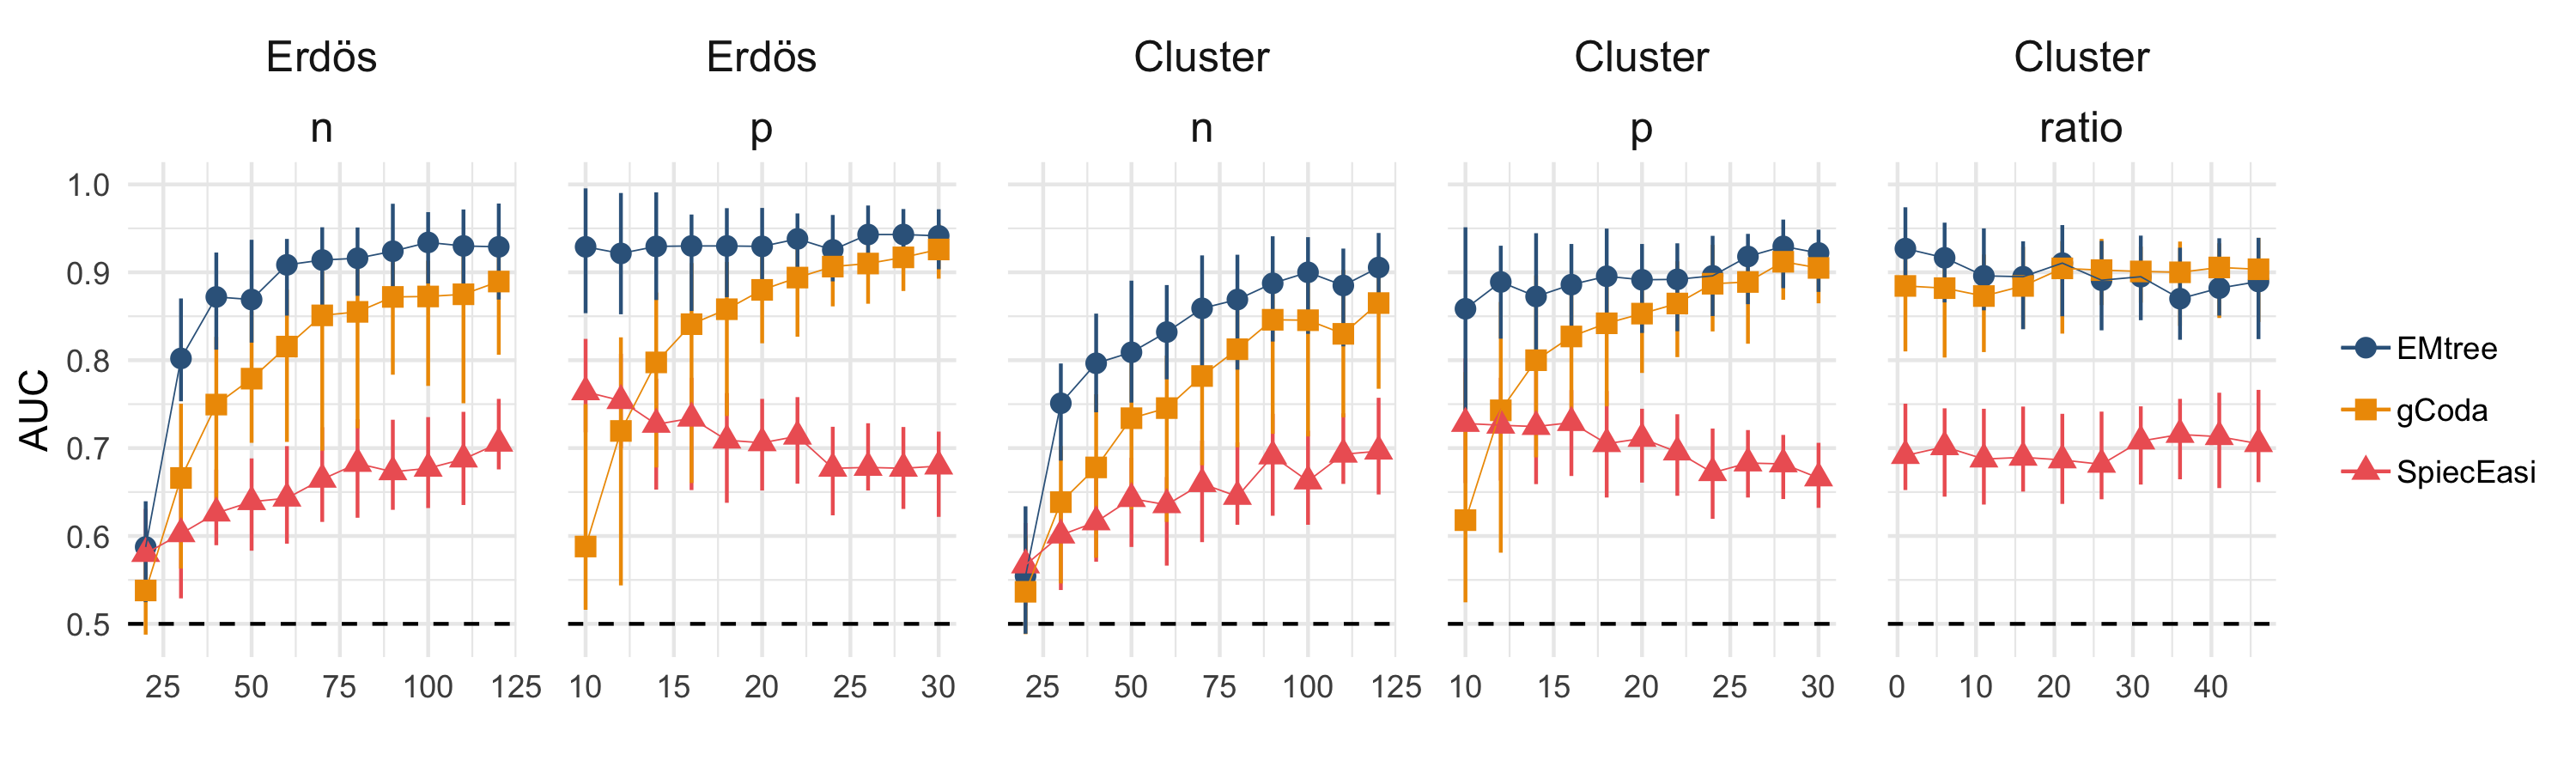
\includegraphics[width=.8\textwidth]{\fignet/MRA19-Fig6top} \\
  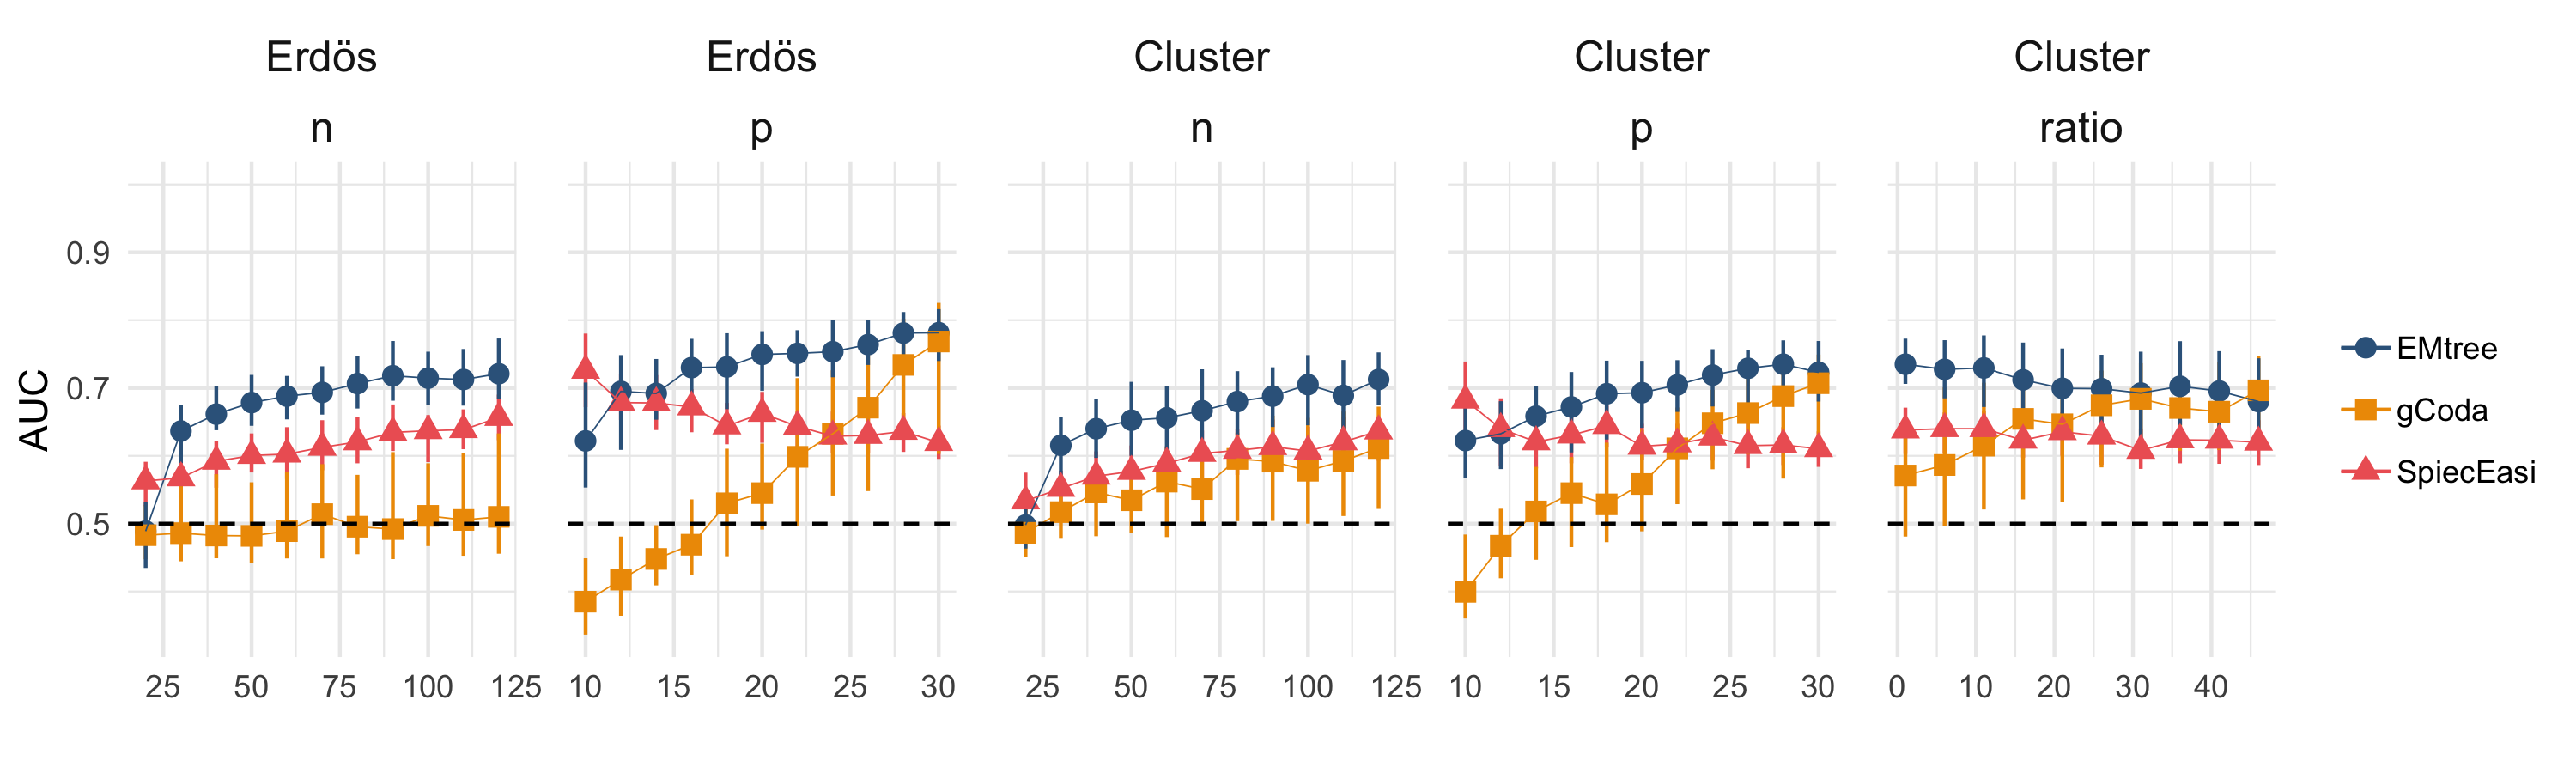
\includegraphics[width=.8\textwidth]{\fignet/MRA19-Fig6bottom} 
  \end{center}

  \ra the tree-shaped assumption does not alter the performances
}

%====================================================================
\frame{\frametitle{Results for the Fatala river} 

  \paragraph{Inferred networks.} 
  $$
  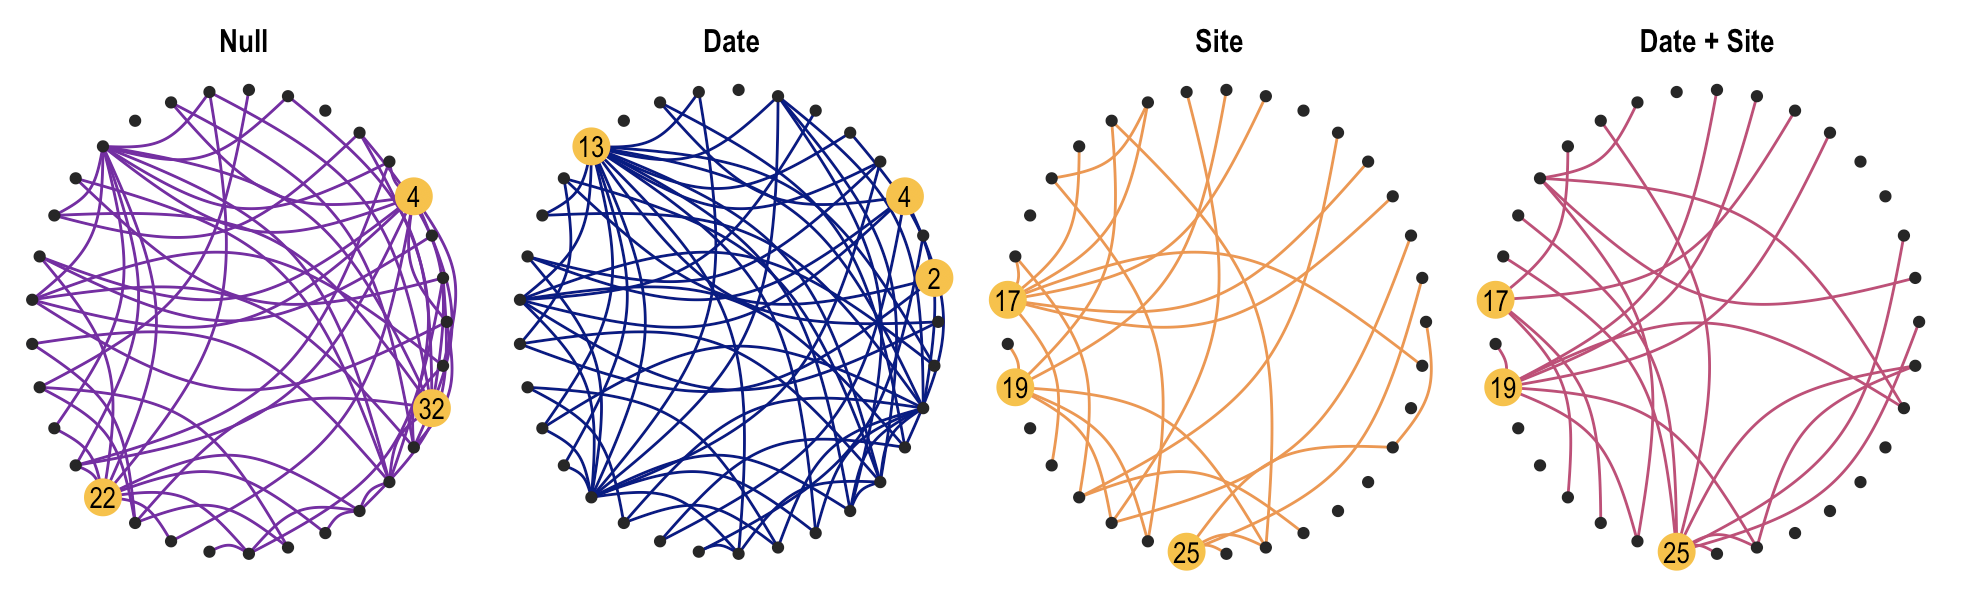
\includegraphics[width=.9\textwidth]{\fignet/MRA19-Fig8} 
  $$
  
  \bigskip \bigskip 
  \paragraph{Some comments.} 
  \begin{itemize}
   \item Accounting for covariates has a dramatic effect on the inferred network
   \item Resampling (StARS \refer{LRW10}) is needed for robustness
   \item Nobody knows the truth (network inference = highly unsupervised problem)
  \end{itemize}

}
%====================================================================
%====================================================================
\section{Spread of an 'epidemic'}
\frame{\frametitle{Outline} \tableofcontents[currentsection]}
%====================================================================
\frame{\frametitle{Susceptible-Infected-Susceptible (SIS) model} 

  \paragraph{Data.} $n$ times, $p$ individuals
  $$
  Y_{tj} = 
  \left\{ \begin{array}{rl}
  1 & \text{if individual $j$ is infected at time $t$} \\
  0 & \text{otherwise}
    \end{array} \right.
  $$
  \ra Complete observations
  
  \bigskip \bigskip 
  \paragraph{Model.} At each time $t$, each node $k$ 
  \begin{itemize}
    \item picks up a parent with probability $\propto \; \beta_{jk}$ and, 
    \item denoting $\psi_{jk}^t = \Pr\{Y_{t+1, k} \mid Y_{t, k}, Y_{t, j}\}$, it evolves according to
    $$
    \begin{array}{cc|cc}
      \multicolumn{2}{c|}{\psi_{jk}^t} & Y_{t+1, k} = 0 & Y_{t+1, k} = 1 \\
      \hline
      Y_{t, k} = 1 & Y_{t, j} = 1 & e & 1-e \\
      Y_{t, k} = 1 & Y_{t, j} = 0 & e & 1-e \\
      Y_{t, k} = 0 & Y_{t, j} = 1 & 1-c & c \\
      Y_{t, k} = 0 & Y_{t, j} = 0 & 1 & 0 
    \end{array}
    $$ 
  \end{itemize}
  \begin{itemize}
   \item $c =$ contamination rate
   \item $e =$ extinction rate (become susceptible again)
  \end{itemize}

}

%====================================================================
\frame{\frametitle{A tree-shaped path} 

  Adding a fictitious root $\Delta$ (at time 0), a path is a tree $T = (T^1, \dots, T^{n-1})$:
  $$
  \includegraphics[width=.6\textwidth]{\fignet/BSR19-Fig1}
  $$
  
  \bigskip \pause
  Define $\Tcal_\Delta$ the set of oriented spanning tree
  \begin{itemize}
   \item over the nodes $\Delta \cup \{(t, k): 1 \leq t \leq n, 1 \leq k \leq p\}$,
   \item rooted in $\Delta$,
   \item with edges $\Ecal(T) \subset \{((t-1, j), (t, k)), j \neq k\}$
  \end{itemize}
  \ra $\Tcal_\Delta =$ set of spanning trees going 'forward' in time ($|\Tcal_\Delta| = (p-1)^{p(n-1)}$)
}

%====================================================================
\frame{\frametitle{Mixture model} 

  \paragraph{Likelihood.} Denote $\theta = (\beta, e, c)$
  \begin{align*}
    p_\theta(Y) 
      & = \sum_{T \in \Tcal_\Delta} p_\beta(T) p_{e, c}(Y \mid T) 
      & = \sum_{T \in \Tcal_\Delta} \prod_{t=1}^{n-1} p_\beta(T^t) p_{e, c}(Y^t \mid Y^{t-1}, T^t) \\
      & = B^{-1} \sum_{T \in \Tcal_\Delta} \prod_{t=1}^{n-1} \prod_{(j, k) \in T^t} \beta_{jk} \psi_{jk}^t
  \end{align*}
  
  \bigskip \pause 
  \begin{itemize}
   \item Mixture model over all possible epidemic paths (path averaging)
   \item Likelihood: Same sum-product form, but over $\Tcal_\Delta$ only. Denoting 
   $$
   W_{jk}^t = \beta_{jk} \psi_{jk}^t
   $$ 
   we end up with simpler form of the matrix-tree theorem.
  \end{itemize}

}


%====================================================================
\frame{\frametitle{An easy situation} 

  \begin{tabular}{lll}
    \begin{tabular}{p{.015\textwidth}}
      $W =$
    \end{tabular}
    &
    \begin{tabular}{l}
      \includegraphics[width=.5\textwidth]{\fignet/BSR19-Fig2p}
    \end{tabular}
   &
   \begin{tabular}{p{.5\textwidth}}
    \paragraph{Matrix-tree:} ~\\
    ~\\
    $
    \Delta(W)^{00} = \prod_{t, j} \left(\sum_k \beta_{jk} \phi_{jk}^t\right)
    $ \\
    ~ \\
    \ra computable in $O(np^2)$
   \end{tabular}
  \end{tabular}
}

%====================================================================
\frame{\frametitle{Inference} 

  \paragraph{EM algorithm.} \refer{BSR19}
  \begin{itemize}
   \item M step: update of $\widehat{\beta}_{jk}$, $\widehat{e}$ and $\widehat{c}$
   \item E step: calculation of $\Pr\{(j, k) \in T^t \mid Y\}$ and $B$ 
   \end{itemize}
   \ra By products: edge probabilities
   $$
   \Pr\{(j, k) \in T^t \mid Y\}, \qquad
   \Pr\{\exists t: (j, k) \in T^t \mid Y\}
   $$

  \bigskip \bigskip \pause
  \paragraph{Alternatives.}
  \begin{itemize}
  \item Bayesian inference can be carried out for $e$ an $c$
  \item In practice, iterating the EM steps does not improve the performances
  \item Observing multiple waves of the epidemic (even over a shortest time-range) improves the accuracy (see next)
  \end{itemize} 
}

%====================================================================
\frame{\frametitle{Simulations: AUC} 

  \begin{tabular}{cc}
    \begin{tabular}{p{.35\textwidth}}
      \paragraph{Design:} \\
      ~ \\
      $p = 20$ nodes \\
      ~ \\
      ER = Erd\"os, \\
      PA = preferential attachment \\
      ~\\
      $e = .05$ \\
      ~\\
      \emphase{uW}: one wave ($n = 200$) \\
      \emphase{mW}: ten waves ($n = 20$) \\
      ~ \\
      \emphase{s}: forcing edge probabilities to be symmetric
    \end{tabular}
    &
    \hspace{-.05\textwidth}
    \begin{tabular}{p{.6\textwidth}}
      \includegraphics[width=.55\textwidth]{\fignet/BSR19-Fig3}
    \end{tabular}   
  \end{tabular}

}

%====================================================================
\frame{\frametitle{Illustration: Seed exchange network} 

  \begin{tabular}{cc}
    \begin{tabular}{p{.4\textwidth}}
      \paragraph{Question:} decipher the social structure underlying the way farmers exchange seeds from one season to another \\
      \ra $Y_{ti}^h =1$ if farmer $i$ holds variety $h$ at time $t$.\\
      ~ \\
      \paragraph{Telangana region data:}\
      ~ \\
      $p = 127$ farmers \\
      $n = 3$ years \\
      14 seed varieties (waves) \\
      \\
      More exchanges \\
      \ra within the same caste \\
      \ra within the same village \\
      \ra from younger to older
    \end{tabular}
    & 
    \begin{tabular}{c}
      \includegraphics[width=.5\textwidth]{\fignet/BSR19-Fig4} \\
      Most probable donor for each farmer
    \end{tabular}
  \end{tabular}
}

%====================================================================
%====================================================================
\section*{Conclusion}
%====================================================================
\frame{\frametitle{Conclusion} 

  \paragraph{Tree shaped mixtures}
  \begin{itemize}
   \item Flexible model for multivariate distributions
   \item Base on a mixture with exponentially many components ($p^{p-2}$)
   \item Giving access to edge probability 
   \item At a low computational cost
  \end{itemize}
  
  \bigskip \pause
  \paragraph{Extensions}
  \begin{itemize}
   \item Network comparison or network changes along time \refer{ScR17}
   \item S-I-S model can be extended to more that two states (e.g. S-I-R models)
   \item Tree-shaped mixtures can be used to infer missing nodes \refer{RAR18}
  \end{itemize}
  
  \bigskip \pause
  \paragraph{Some questions}
  \begin{itemize}
    \item Which distributions are well approximated by tree-shaped mixtures?
    \item Numerical issues arise for large $p$ or $n$ (use tempering?)
  \end{itemize}
}

%====================================================================
\frame[allowframebreaks]{ \frametitle{References}
  {%\footnotesize
   \tiny
   \bibliography{/home/robin/Biblio/BibGene}
%    \bibliographystyle{/home/robin/LATEX/Biblio/astats}
   \bibliographystyle{alpha}
  }
}

%====================================================================
\backupbegin
%====================================================================
%====================================================================
\frame{\frametitle{Change-point detection \refer{ScR17}} 

  \paragraph{Data:} $N = 67$ time points, $p = 11$ genes, four expected regions \refer{LBD10}

  \pause \bigskip
  Posterior probability of change-points:
  $$
  \includegraphics[width=.7\textwidth]{\figchp/ScR16-Fig8-chgpt_EMP_ap10_au1}
  $$
  \pause
  Inferred networks:
  $$
  \includegraphics[width=.8\textwidth]{\figchp/ScR16-Fig9-network_seuil02}
  $$

}

%====================================================================
\backupend
%====================================================================

%====================================================================
%====================================================================
\end{document}
%====================================================================
%====================================================================
  
  \hspace{-.025\textwidth}
  \begin{tabular}{cc}
    \begin{tabular}{p{.5\textwidth}}
    \end{tabular}
    & 
    \hspace{-.02\textwidth}
    \begin{tabular}{p{.5\textwidth}}
    \end{tabular}
  \end{tabular}

